\documentclass[12pt]{Homework}

% Changed from \usepackage{prelude}
\usepackage{preamble}
\usepackage{amssymb}
\usepackage{enumitem}
\usepackage{mathrsfs}
\def\upint{\mathchoice%
    {\mkern13mu\overline{\vphantom{\intop}\mkern7mu}\mkern-20mu}%
    {\mkern7mu\overline{\vphantom{\intop}\mkern7mu}\mkern-14mu}%
    {\mkern7mu\overline{\vphantom{\intop}\mkern7mu}\mkern-14mu}%
    {\mkern7mu\overline{\vphantom{\intop}\mkern7mu}\mkern-14mu}%
  \int}
\def\lowint{\mkern3mu\underline{\vphantom{\intop}\mkern7mu}\mkern-10mu\int}
\usepackage[mathscr]{euscript}
\usepackage{comment}
\usepackage{MnSymbol}
\usepackage{tikz,float}
\usepackage{bbding}
\renewcommand\qedsymbol{\Peace}
\newcommand\placeqed{\nobreak\enspace\Peace}
\usepackage{tikz-cd}
\usepackage{graphicx}
\usepackage{mathtools}
\usepackage{caption, threeparttable}
\usepackage{halloweenmath}
\newcommand{\contradiction}{\null\hfill\large{$\mathghost$}\normalsize}
\newcommand{\im}{\mathscr{I}\text{m}}
\newcommand{\re}{\mathscr{R}\text{e}}
\newcommand{\res}{\text{Res}}

\name{Kayla Orlinsky}
\course{Complex Analysis Exam}
\term{Spring 2018}
\hwnum{Spring 2018}

\begin{document}

\begin{problem} $\,$
Show that there is no holormophic function $f$ in $\mathbb{D}=\{|z|<1\}$ so that $|f(z_n)|\to\infty$ whenever $|z_n|\to 1$ $(z_n\in\mathbb{D})$.
\end{problem}


\begin{solution}$\,$
Let $f$ be holomorphic in $\mathbb{D}$. Assume $|f(z_n)|\to\infty$ whenever $|z_n|\to 1$. Since zeros are isolated, there at most countably many inside $\mathbb{D}$.

However, if there are infinitely many zeros, then there cannot exist an accumulation point inside $\mathbb{D}$, otherwise $f\equiv 0$ by the identity theorem. But then there would exist a limit point inside $\overline{\mathbb{D}}$ and since the limit point is not in $\mathbb{D}$, its on the boundary. Thus, the sequence of zeros of $f$ $\{a_n\}$, satisfies that $|a_n|\to1$ and $|f(a_n)|\to0$, contradicting the hypothesis. 


Therefore, $f$ can have only finitely many zeros inside $\mathbb{D}$.

Let $f(z)=(z-a_1)\cdots(z-a_k)g(z)$ for $g(z)$ analytic in $\mathbb{D}$ and never zero. Then $$\frac{f(z)}{(z-a_1)\cdots(z-a_k)}=g(z)$$ which is holomorphic and nonzero. Thus, $\frac{1}{g}$ is holomorphic and nonzero.

Since $a_i\in\mathbb{D}$, for any sequence $\{z_n\}$ with $|z_n|\to 1$, for all $\varepsilon>0$, there exists $N$ so $|z_n-a_i|\ge\varepsilon$ for all $n\ge N$. Namely, since $f$ explodes near the boundary of $\mathbb{D}$, so too must $g$.

Therefore, $\frac{1}{|g(z_n)|}\to0$ whenever $|z_n|\to1$ so by the maximum modulus principle, implies $\frac{1}{g}\equiv0$. Clearly a contradiction.

Thus, $g$ cannot exist and so neither can $f$.
\end{solution}
\newpage



\begin{problem} $\,$
Assume that $f$ is analytic in the unit disk $\mathbb{D}=\{z:|z|<1\}.$ Prove that $f$ is odd if and only if all the terms in the Taylor series for $f$ at $z_0=0$ have only odd powers.
\end{problem}

\begin{solution}$\,$

\boxed{\implies} Assume $f$ is odd. Then $f(-z)=-f(z)$ for all $z\in\mathbb{D}$. Since $f$ is analytic, it has a taylor series at $0$. Thus, $$f(z)=\sum_{n=0}^\infty a_nz^n\qquad z\in\mathbb{D}.$$

Now, for $r>0$ small, we get that \begin{align*}
    a_{2n}&=\frac{f^{2n}(0)}{(2n)!}\\
    &=\frac{1}{2\pi i}\int_{|z|=r}\frac{f(z)}{z^{2n+1}}dz\\
    &=\frac{1}{2\pi}\int_0^{2\pi}\frac{f(re^{i\theta})}{r^{2n}e^{2ni\theta}}d\theta\qquad z=re^{i\theta}\\
    &=\frac{1}{2\pi}\left[\int_0^\pi\frac{f(re^{i\theta})}{r^{2n}e^{2ni\theta}}+\int_\pi^{2\pi}\frac{f(re^{i\theta})}{r^{2n}e^{2ni\theta})}\right]\\
    &=\frac{1}{2\pi}\left[\int_0^\pi\frac{f(re^{i\theta})}{r^{2n}e^{2ni\theta}}+\int_0^\pi\frac{f(re^{i(\theta-\pi)})}{r^{2n}e^{2ni(\theta-\pi)}}\right]\\
    &=\frac{1}{2\pi}\left[\int_0^\pi\frac{f(re^{i\theta})}{r^{2n}e^{2ni\theta}}+\int_0^\pi\frac{f(-re^{i\theta})}{r^{2n}e^{2ni\theta}}\right]\\
    &=\frac{1}{2\pi}\left[\int_0^\pi\frac{f(re^{i\theta})}{r^{2n}e^{2ni\theta}}+\int_0^\pi\frac{-f(re^{i\theta})}{r^{2n}e^{2ni\theta}}\right]\\
    &=0
\end{align*} for all $n$ since $f$ is odd.

Thus, $$f(z)=\sum_{n=0}^\infty a_{2n+1}z^{2n+1}.$$

\boxed{\impliedby} This clear. Since $f$ is analytic, it has a taylor series at $0$. Thus, $$f(z)=\sum_{n=0}^\infty a_nz^n=\sum_{n=0}^\infty a_{2n+1}z^{2n+1}$$ since all the terms in the taylor series have only odd powers.

Thus, $$f(-z)=\sum_{n=0}^\infty a_{2n+1}(-z)^{2n+1}=\sum_{n=0}^\infty (-1)^{2n+1}a_{2n+1}z^{2n+1}=-\sum_{n=0}^\infty a_{2n+1}z^{2n+1}=-f(z).$$ So $f$ is odd.
\end{solution}
\newpage




\begin{problem} $\,$
Evaluate $$\int_{-\infty}^\infty\frac{\cos(2x)}{x^2+1}dx$$
\end{problem}


\begin{solution}$\,$
We examine $\displaystyle\int\frac{e^{i2z}}{z^2+1}dz$ and use ``Ol' Faithful'' with the origin. Namely, the contour around the upper half plane.

\begin{center}
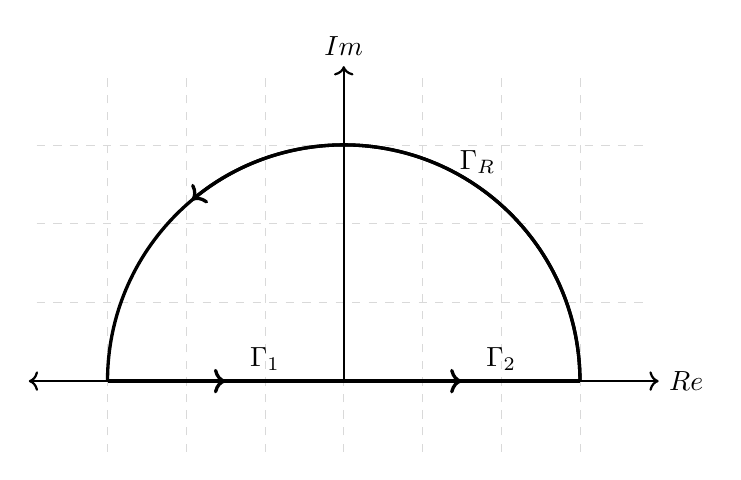
\begin{tikzpicture}
\draw[help lines, color=gray!30, dashed] (-3.9,-0.9) grid (3.9,3.9);
\draw[->,very thick] (3,0) arc (0:130:3cm);
\draw[very thick] (3,0) arc (0:180:3cm) node[above,yshift=2.5cm,xshift=4.7cm]{$\Gamma_R$};
\draw[->,very thick] (0,0) -- (1.5,0);
\draw[very thick] (0,0) -- (3,0) node[above,yshift=0cm,xshift=-1cm]{$\Gamma_2$};
\draw[->,very thick] (-3,0) -- (-1.5,0);
\draw[very thick] (-3,0) -- (0,0) node[above,yshift=0cm,xshift=-1cm]{$\Gamma_1$};
\draw[<->, thick] (-4,0)--(4,0) node[right]{$Re$};
\draw[->, thick] (0,0)--(0,4) node[above]{$Im$};
\end{tikzpicture}
\end{center}

Let \begin{align*}
    I_1&=\int_{\Gamma_1}\frac{e^{2iz}}{z^2+1}dz\\
    I_2&=\int_{\Gamma_2}\frac{e^{2iz}}{z^2+1}dz\\
    I_R&=\int_{\Gamma_R}\frac{e^{2iz}}{z^2+1}dz
\end{align*}

Now, we note that $\cos(-2x)=\cos(2x)$ since $\cos$ is an even real function and so $$\int_{-\infty}^\infty\frac{\cos(2x)}{x^2+1}dx=2\int_0^\infty\frac{\cos(2x)}{x^2+1}dx$$

Then, we note that \begin{align*}
    I_1+I_2&=\int_{\Gamma_1}\frac{e^{2iz}}{z^2+1}dz+\int_{\Gamma_2}\frac{e^{2iz}}{z^2+1}dz\\
    &=\int_{-R}^0\frac{e^{2ix}}{x^2+1}dx+\int_0^R\frac{e^{2ix}}{x^2+1}dx\\
    &=\int_R^0-\frac{e^{-2ix}}{x^2+1}dx+\int_0^R\frac{e^{2ix}}{x^2+1}dx\\
    &=\int_0^R\frac{e^{-2ix}}{x^2+1}dx+\int_0^R\frac{e^{2ix}}{x^2+1}dx\\
    &=\int_0^R\frac{e^{2ix}+e^{-2ix}}{x^2+1}dx\\
    &=\int_0^R\frac{2\cos(2x)}{x^2+1}dx\\
    &=2\int_0^R\frac{\cos(2x)}{x^2+1}dx
\end{align*}

Finally, \begin{align*}
    |I_R|&=\left|\int_{\Gamma_R}\frac{e^{2iz}}{z^2+1}dz\right|\\
    &\le\int_{\Gamma_R}\frac{|e^{2iz}|}{|z^2+1|}d|z|\\
    &\le\int_{\Gamma_R}\frac{e^{-2\im(z)}}{|z|^2-1}d|z|\\
    &\le\int_0^\pi\frac{Re^{-2R\sin\theta}}{R^2-1}d\theta \qquad z=Re^{i\theta}\\
    &=\frac{R}{R^2-1}\int_0^\pi e^{-2R\sin\theta} d\theta\\
    &\le \frac{R}{R^2-1}\int_0^\pi d\theta\qquad \sin\theta\ge 0\text{ on upper half plane}\\
    &=\frac{\pi R}{R^2-1}\to0\qquad R\to\infty
\end{align*}

Therefore, by the residue theorem, 
\begin{align*}
    2\pi i\res_{z=i}\frac{e^{2iz}}{z^2+1}&=2\pi i\frac{e^{-2}}{i+i}\\
    &=\frac{\pi}{e^2}\\
    &=\lim_{R\to0}(I_1+I_2+I_R)\\
    &=2\int_0^\infty\frac{\cos(2x)}{x^2+1}dx\\
    \int_{-\infty}^\infty\frac{\cos(2x)}{x^2+1}dx&=\frac{\pi}{e^2}
\end{align*}
\end{solution}
\newpage





\begin{problem} $\,$
Let $\mathbb{D}=\{|z|<1\}$ be the open unit disk and $\overline{\mathbb{D}}$ its closure. Let $f:\mathbb{D}\to\mathbb{C}$ be analytic on $\mathbb{D}$ and continuous on $\overline{\mathbb{D}}$. Assume that $f$ only takes real values on $\partial\overline{\mathbb{D}}=\{|z|=1\}.$ Prove that $f$ is constant.
\end{problem}


\begin{solution}$\,$
Now, since $f$ is analytic $\im(f(z))$ is a harmonic function in the disk which is continuous ont he boundary of the unit disk. Thus, by the maximimum modulus principle, $|\im(f(z))|$ has to reach a maximum on $\partial\overline{\mathbb{D}}$. 

However, \begin{align*}
    |\im(f(z))|&\le\sup_{z\in\partial\overline{\mathbb{D}}}|\im(f(z))|\\
    &=\sup_{z\in\partial\overline{\mathbb{D}}}|\frac{1}{2}(f(z)-\overline{f(z)})|\\
    &=\sup_{z\in\partial\overline{\mathbb{D}}}|\frac{1}{2}(f(z)-f(z))|\qquad f(z)\in\mathbb{R}\text{ whenever }z\in\partial\overline{\mathbb{D}}\\
    &=0
\end{align*}

Thus, $f$ is a real function. 

However, Cauchy-Riemann then implies that $f=u+iv=u$ must be a constant since $u$ must be a constant because $u_x=v_y=0$ and $u_y=-v_x=0$.

Thus, $f$ is a real constant.
\end{solution}


\end{document}
 